
\documentclass[12pt,journal,compsoc]{IEEEtran}

\ifCLASSOPTIONcompsoc
\fi

\ifCLASSINFOpdf
\fi

\newcommand\MYhyperrefoptions{bookmarks=true,bookmarksnumbered=true,
pdfpagemode={UseOutlines},plainpages=false,pdfpagelabels=true,
colorlinks=true,linkcolor={black},citecolor={black},urlcolor={black},
pdftitle={Bare Demo of IEEEtran.cls for Computer Society Journals},%<!CHANGE!
pdfsubject={Typesetting},%<!CHANGE!
pdfauthor={Michael D. Shell},%<!CHANGE!
pdfkeywords={Computer Society, IEEEtran, journal, LaTeX, paper,
             template}}%<^!CHANGE!
\hyphenation{op-tical net-works semi-conduc-tor}



\usepackage{tikz}
\usetikzlibrary{shapes.geometric, arrows}
\tikzstyle{startstop} = [rectangle, rounded corners, minimum width=3cm, minimum height=1cm,text centered, draw=black, fill=red!30]
\tikzstyle{io} = [trapezium, trapezium left angle=70, trapezium right angle=110, minimum width=3cm, minimum height=1cm, text centered, draw=black, fill=blue!30]
\tikzstyle{process} = [rectangle, minimum width=3cm, minimum height=1cm, text centered, draw=black, fill=orange!30]
\tikzstyle{decision} = [diamond, minimum width=3cm, minimum height=1cm, text centered, draw=black, fill=green!30]
\tikzstyle{arrow} = [thick,->,>=stealth]
\tikzstyle{line}=[
	draw, -latex',
]
\usepackage{enumerate}
\usepackage{amsmath}
\usepackage{hyperref}
\usepackage{url}


\begin{document}
\title{Graph-Based Ant Colony Simulation}

\author{Shao-Hsuan Chu
        Meng-Ting Wu,
        Hung-I Lin,
        and~Ju-Ting Chen}% <-this % stops a space


% The paper headers
\markboth{January~2021}%
{Shell \MakeLowercase{\textit{et al.}}: Graph-Based Ant Colony Simulation}

\IEEEtitleabstractindextext{%
\begin{abstract}

Ant Colony Optimization(ACO) algorithm is a popular metaheuristic algorithms based on the behaviors of animals. The pheromone ants leave on their trails is especially useful to solve route-finding problems. In this paper, some rules of the algorithm are modified to make it closer to biological behaviors in nature. We build our simulation on a modified directed acyclic graph, which prevents an ant from following its own trail and enables us to observe in discrete configurations. In order to give a better view of the nature-inspired techniques and cross-platform compability, we implement the artificial colony in JavaScript/p5js.
\thanks{Live demo: \url{https://ernestchu.github.io/ACO-Web/}}
\thanks{Source code: \url{https://github.com/ernestchu/ACO-Web}}


\end{abstract}

% Note that keywords are not normally used for peerreview papers.
\begin{IEEEkeywords}
Swarm Intelligence, Metaheuristics, ACO, Graph Theory.
\end{IEEEkeywords}}


% make the title area
\maketitle

\IEEEdisplaynontitleabstractindextext

\IEEEpeerreviewmaketitle



\section{Introduction}


\IEEEPARstart{S}{warm} Intelligence based algorithm is a technique which simulates the behavior of creatures in nature. This concept is used widely in Artificial Intelligence. Boids, an early proposed concept developed by Craig Reynolds in 1986, is an Artificial Life program which mimics the behavior of flock of birds. Some metaheuristic algorithms are greatly inspired by biological behaviors. Ant Colony Optimization is one of the most popular metaheuristics, introduced by Marco Dorigo, which has several individual ants as agents to search for a better solution in the search space.

\subsection{Introduction of Ant Colony Optimization}

Bionics, which refers to the study of mechanical systems that function like living organisms. Marco Dorigo et al.[1] takes the idea of Bionics to the computer world. The paper points out the connection between the foraging behavior of ants and the combinatorial optimization problems, for instance, the famous Travelling Salesman Problem(TSP). The pheromone left by ants to find food is the key component of the optimization algorithm. It can be divided into two parts in the first ACO algorithm, Ant System(AS), pheromone update and route selection.


\subsubsection{Pheromone Update}
The paper states that pheromone are left by the ants who found food, and the other ants can follow their path to find the food. Like the smell in our world, pheromone evaporates over time. Therefore, an evaporation rate $\rho$ is imposed on the existing pheromone $\tau$.
\[\tau_{ij}\leftarrow(1-\rho)\cdot\tau_{ij}+\sum\limits_{k=1}^{m}\Delta\tau_{ij}^{k}\]
where $\tau_{ij}$ stands for the pheromone on the route from point $i$ to point $j$ \\
$\Delta\tau_{ij}^{k}$ is defined by
\[\Delta\tau_{ij}^{k}=\begin{cases} Q/L_{k} &\mbox{if ant k used edge (i,j)in its tour} \\
0 & \mbox{otherwise,}\end{cases}\]
where $Q$ is a constant, $L_{k}$ is the length of route. It shows that the intensity of pheromone is inversely proportional to the length of route, which eventually makes ants to take the shortest route.
\subsubsection{Route Selection}
The paper claims that ants select the next points by a stochastic mechanism.
When ant $k$ is in point $i$ and has the partial solution $s^{p}$, the probablility of going to point j is
\[p_{ij}^{k}=\begin{cases} {\tau_{ij}^{\alpha}\eta_{ij}^{\beta}\over \sum\nolimits_{c_{ij}\in {\bf N}(s^{p})}\tau_{il}^{\alpha}\cdot\eta_{1l}^{\beta}} &\mbox{if }\ c_{ij}\in {\bf N}(s^{p}), \\
0 & \mbox{otherwise,}\end{cases}\]
where $\alpha$ and $\beta$ controll the importance of pheromone versus $\eta_{ij}$, which is given by.
\[\eta_{ij}={1\over d_{ij}},\]
Where $1\over d_{ij}$ is the distance between points $i, j$.
Intuitively, the shorter route means the ants comes back quicker, which attract the other ants since there's no other ants come back from another route. As a result, those ants attracted reinforce the intensity of the pheromone on the route they take.

\section{The Ant Colony Simulation}
At the start of the program, a fixed number of ants is summoned to the world. The world is essentially a directed acyclic graph (DAG) with some exceptions. The ants can visit reachable vertices and leave the pheromone on the edges of the graph. While leaving the pheromone, the ants also record the edges they've taken, so they can go back to the nest as long as they found food or there's no reachable vertex. The basic workflow of every ants in the program is as follow: \\

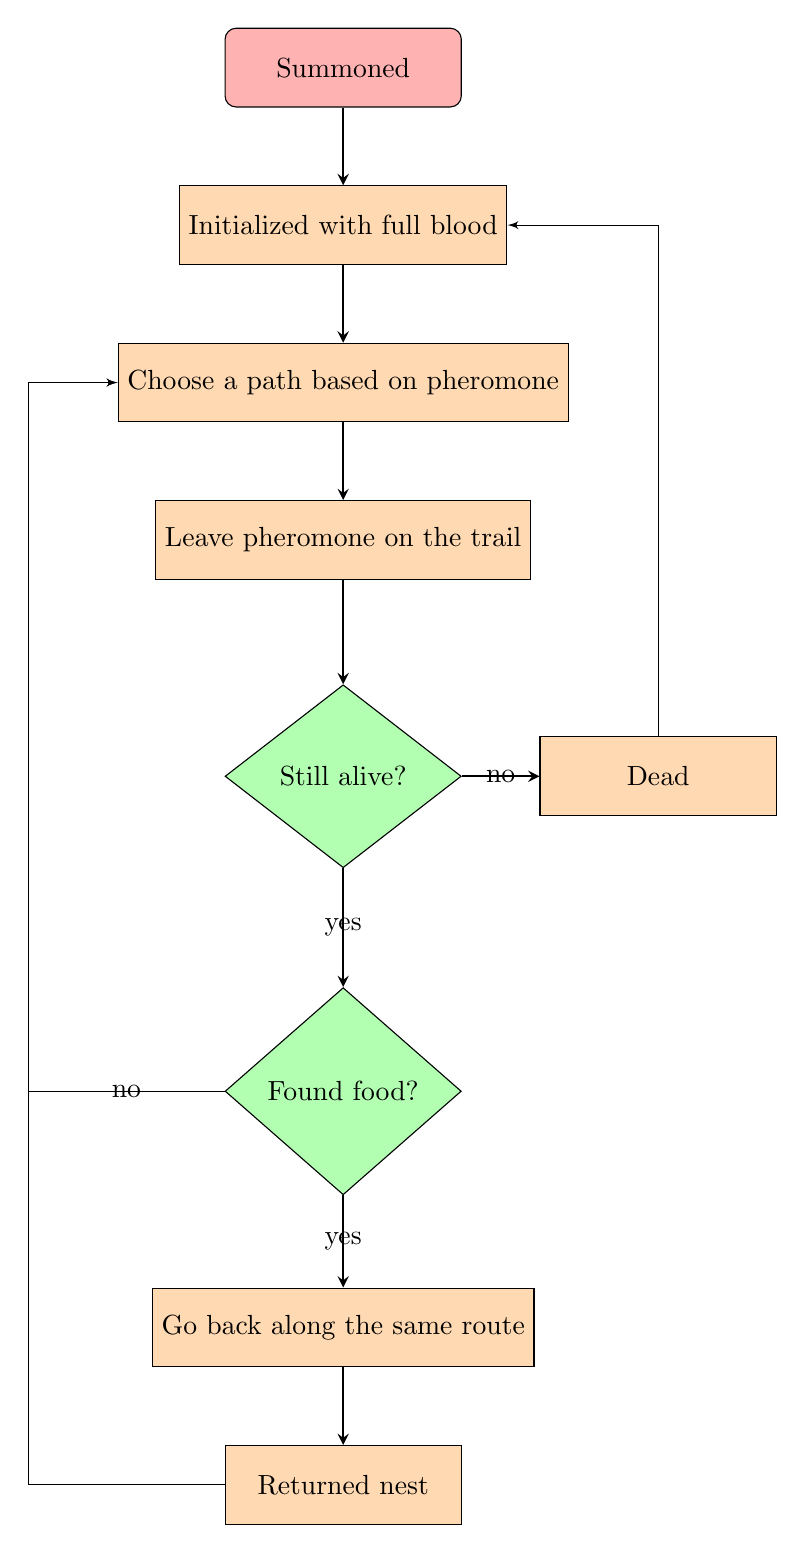
\begin{tikzpicture}[node distance=2cm]
\node (start) [startstop] {Summoned};
\node (pro1) [process, below of=start] {Initialized with full blood};
\node (pro2) [process, below of=pro1] {Choose a path based on pheromone};
\node (pro3) [process, below of=pro2] {Leave pheromone on the trail};
\node (dec1) [decision, below of=pro3, yshift=-1cm] {Still alive?};
\node (pro4) [process, below of=pro3, xshift=4cm, yshift=-1cm] {Dead};
\node (dec2) [decision, below of=dec1, yshift=-2cm] {Found food?};
\node (pro5) [process, below of=dec2, yshift=-1cm] {Go back along the same route};
\node (pro6) [process, below of=pro5] {Returned nest};

\draw [arrow] (start) -- (pro1);
\draw [arrow] (pro1) -- (pro2);
\draw [arrow] (pro2) -- (pro3);
\draw [arrow] (pro3) -- (dec1);
\draw [arrow] (dec1) -- node {yes} (dec2);
\draw [arrow] (dec1) -- node {no} (pro4);
\path[line] (pro4) |-  (pro1);
\path[line] (dec2) -- node {no} ++(-4cm, 0) |- (pro2);
\draw [arrow] (dec2) -- node {yes} (pro5);
\draw [arrow] (pro5) -- (pro6);
\path[line] (pro6) -- ++(-4cm, 0) |- (pro2);
\end{tikzpicture}

The ants are initialized with full blood, which decrements in a constant rate. When an ant has no blood, it's dead and it a new ant will be summoned immediately. So in the program implementation, we can just reinitialize the very ant. Also, the world contains not only ants but food and obstacles. We will elaborate below.

\subsection{The Modified DAG}
In our modified DAG, the nest, i.e. the statring vertex, is at the upper left most and each vertex has directed edges to the lower-right, right, lower verticess, which follows the rules of DAG. However, for the purpose of exploring upper right and lower left of the world, we added the connections to the directions respectively as the following figure illustrated.\\\\
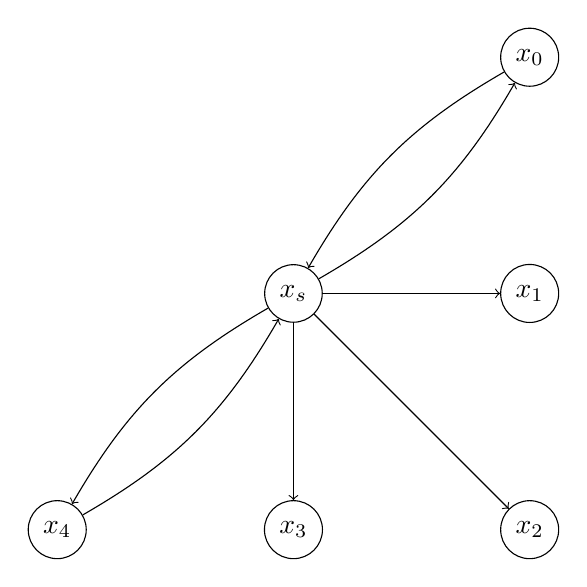
\begin{tikzpicture}[node distance={30mm}, main/.style = {draw, circle}]
\node[main] (-1) {$x_s$};
\node[main] (1) [right of=-1] {$x_1$};
\node[main] (0) [above of=1] {$x_0$};
\node[main] (2) [below of=1] {$x_2$};
\node[main] (3) [below of=-1] {$x_3$};
\node[main] (4) [left of=3] {$x_4$};

\draw[->] (-1) -- (1);
\draw[->] (-1) -- (2);
\draw[->] (-1) -- (3);
\draw[->] (-1) to [out=30,in=240] (0);
\draw[->] (0) to [out=210,in=60] (-1);
\draw[->] (-1) to [out=210,in=60] (4);
\draw[->] (4) to [out=30,in=240] (-1);
\end{tikzpicture}
\\\\
Where $x_s$ represents the starting vertex and the bidirectional edge is one edge instead of two seperated edges. This auxiliary connections violet the rules of DAG and lead to the infinity cycles in which the ants would be trapped. Supposed an ant visit $x_0$ from $x_s$. Because of the pheromone affinity, the ant would have high possibility taking the edge which it just took and goes back to the vertex where it came from, and so on and so forth. To prevent this, we added a constraint in our program, which forbids the ants from taking the bidirectional edge again.

\subsection{The pheromone affinity}
We know that an ant makes its decision on the edges based on the pheromone they last. The probablility $p_{ij}$ of each vertex $j$ from vertex $i$ is given by
\[p_{ij}=\begin{cases} p_{pher}{\tau_{ij}\over \sum\nolimits_{k\in {\bf Adj}(i)}\tau_{ik}}\\ + (1-p_{pher}){1\over\|\bf Adj(i)\|} &\mbox{if }\ j\in {\bf Adj}(i), \\
0 & \mbox{otherwise,}\end{cases}\]
where $\bf Adj(i)$ is a set of reachable vertices from vertex $i$, $\tau_{ij}$ is the pheromone and $p_{pher}$ is the probablility of an ant affected by the pheromone. The ants do not follow the pheromone every time so it's less likely to fall into local optima. In addition, we also remove some reachable vertices in the boundry condition as the ants cannot go out of the world.

\subsection{The Food}
There are there cases that an ant doesn't continue to explore the world and go back to the nest. First, there's no reachable vertices due to either the obstacles or the boundry of the world. Second, the ant died of the hunger, i.e. the blood became zero. Third, they found food. We can consider the constraint of the blood as the longest path an ant is allowed to explore. It also helps the ant colony to find the shortest path toward food easily. When an ant found the food, it's blood gets refilled so it can bring the food back to the nest. In the program, food can be placed dynamically and we can place multiple units of food in the world. Sometimes, the ants would stuck at a local optimal path from the nest to boundry. That's is because the ants leave pheromone as soon as they leaved the nest and when they hit the boundry, they go back without producing pheromone. Even with such configuration, the ants still have chances to stuck at a nest-to-boundry path. It's most likely when they finished a food unit near the boundry. In our program, we provide a button to eliminate all the pheromone in the world, so the ants can search for food randomly again.

\subsection{The Obstacles}
As mentioned above, the reachable vertices can be removed by the obstacles. In our program, obstacles can be placed dynamically on a certain vertex, which disable the very vertex so no ant can visit it. We add the setting of obstacles in order to observe how ant colony acts in an irregular landform. However, we allow the ants to cross the obstacles when they're going back to the nest, which is necessary otherwise they don't know how to get home. In the real world, ants have antenna to communicate with each other, and we believe that this is how ants overcome the dynamic changes of the landform. But we didn't include such setting in our program.


\section{Conclusion And Observation}
Several decades of development in Swarm Intelligence has seen plenty exciting works. The purpose of this research is to visualize the artificial biological behaviors in such algorithms while there are still some space for improvement. We noticed that there're several hyper parameters that matter a lot w.r.t. the operation of the colony, including the decay rate of pheromone, the probablility of being affect by pheromone and the blood decrement rate. We tested several combinations and finally got an presentable outcome. Still, the ants stuck at the local optima sometimes as the world is finite. As state-of-the-art nature-inspired algorithms springing up, we dedicate to implement them in future works.


\ifCLASSOPTIONcaptionsoff
  \newpage
\fi


\begin{thebibliography}{1}


  \bibitem{citekey}
  M. Dorigo, M. Birattari and T. Stutzle,\emph{ "Ant colony optimization"}\hskip 1em plus
  0.5em minus 0.4em\relax in IEEE Computational Intelligence Magazine, vol. 1, no. 4, pp. 28-39, Nov. 2006, doi: 10.1109/MCI.2006.329691.

\end{thebibliography}

\end{document}
